\documentclass[10pt,a4paper]{article}
\usepackage[utf8]{inputenc}
\usepackage{amsmath}
\usepackage{amsfonts}
\usepackage{mathtools}
\usepackage{amssymb}
\usepackage{graphicx}
\usepackage{subcaption}
\usepackage{dsfont}
\usepackage[strict]{changepage}
\usepackage{float}
\usepackage{graphicx}
\usepackage{parskip}
\makeatletter
\newcommand*{\transpose}{%
  {\mathpalette\@transpose{}}%
}
\newcommand*{\@transpose}[2]{%
  % #1: math style
  % #2: unused
  \raisebox{\depth}{$\m@th#1\intercal$}%
}

\author{Adam Jalkemo \texttt{adam@jalkemo.se} \and
Alexander Israelsson \texttt{israelsson.alexander@gmail.com} \and
Emil Westenius \texttt{emil@westenius.se} \and
Jonathan Andersson \texttt{mat11ja1@student.lu.se}
\and 
\\
Supervisor: Gabriel Ingeson}
\begin{document}

\title{Adaptive Friction Compensation}

\maketitle
\pagebreak
\section{Introduction}
In this project a Furuta pendulum process will be used. The Furuta pendulum consists of a pendulum, that is free to rotate in the vertical plane, attached to the end of an horizontally rotating arm that can be controlled. The pendulum will be stabilized in the inverted position using a swing up controller and a top controller. When controlling the pendulum in the top position limit cycles will occur due to friction. By compensating for the friction we aim to stabilize the pendulum, the friction will be estimated using an adaptive method. To do this a Java controller and interface will be implemented and run on a linux computer.
%\begin{figure}[!htb]
%\begin{center}
%\includegraphics[width=1\textwidth]{process.png}
%\caption{The furuta pendulum in the inverted position}
%\label{fig:process}
%\end{center}
%\end{figure}
\section{Program structure}
For our suggested solution we will need one thread for the GUI and one for the controller. To communicate with the Furuta process we will use the analog box normally used during the control labs at LTH. The realtime package from Automatic Control at LTH will be used for communication in the GUI and controller implementation. It will be important to synchronize the controller calculations with the user inputs. A general overview can be seen in figure \ref{fig:uml}.

\begin{figure}[!htb]
\begin{center}
\includegraphics[width=1\textwidth]{notUml.png}
\caption{Overview of the program structure}
\label{fig:uml}
\end{center}
\end{figure}
%% MORe STUFFS??

%ToDo UML AND DESCRIPTION OF CLASSES AND PACKAGES


%Todo what parameters can be changed.
\section{System model}
Due to the non-linear dynamics of the rotating arm and pendulum the modelling of the process becomes complicated. We have used the model given in Lab2 in "Non-linear control" where the model have been simplified with the help of Lagrange theory. The dynamics of the model is then given by:
$$(J_p + Ml^2)(\ddot{\theta} - \dot{\varphi} ^2\sin\theta \cos\theta )+Mrl\ddot{\varphi}\cos\theta-gl(M+m/2)\sin\theta = 0 $$
\begin{equation}
Mrl\ddot{\theta}\cos\theta - Mrl\dot{\theta ^2}\sin\theta + 2(J_p + ml^2 ) \dot{\theta} \dot{\varphi}\sin\theta \cos\theta + (J+mr^2 + Mr^2 + (J_p+ml^2)\sin^2\theta)\ddot{\varphi}=u
\label{eq:model}
\end{equation}
where $\theta$ is the angle of the pendulum, $\varphi$ is the angle of the arm and $u$ is the motor torque on the arm. The states $\theta$, $\dot{\theta}$, $\varphi$ and $\dot{\varphi}$ will all be measured from the process and $u$ will be our control signal. The approximated coefficients are also taken from Lab2 and are given by:
$$l=0.413m \quad  r=0.235m$$
$$M=0.01kg \quad J=0.05kgm^2$$
$$J_p=0.0009kgm^2 \quad m=0.02kg$$
$$ g=9.8$$
Where $l$ is the length of the pendulum, $r$ is the length of the arm, $M$ is the mass of the weight, $J$ is moment of inertia  for pendulum, $J_p$ is the moment of inertia for the arm, $m$ is the mass of the pendulum and $g$ is the gravity constant.
\subsection{Linearization}
The model in \ref{eq:model} is then linearized around
\begin{equation}
x =
\begin{pmatrix}
\theta & \dot\theta & \varphi & \dot\varphi
\end{pmatrix} = 
\begin{pmatrix}
0 & 0 & 0 & 0
\end{pmatrix}
\end{equation}
which yields 
\begin{equation}
\dot{x} = Ax + Bu =
\begin{pmatrix}
0 & 1 & 0  & 0 \\
\frac{bd}{ab-c^2} & 0 & 0 & 0 \\
0 & 0 & 0 & 1 \\
\frac{-cd}{ab-c^2} & 0 & 0 & 0
\end{pmatrix}x
+
\begin{pmatrix}
0 \\
\frac{-cg}{ab-c^2} \\
0 \\
\frac{ag}{ab-c^2}
\end{pmatrix}u
\label{eq:linear}
\end{equation}
where 
$$ a = J_p + M l^2 \qquad b = J + M r^2 + m r^2 $$
$$ c = M r l  \qquad d = l g (M + m/2) $$
This corresponds to the arm fixed at an angle corresponding to zero and the pendulum fixed in the top position. It is in this position that the friction will create oscillations and where the adaptive friction compensation will be applied.
\subsection{Discretization}
The linearized model is then discretized using ZoH. A simplified ZoH method have been implemented in java which makes it possible to change the sample time online. For the most part a sample time of $h=0.01$ have been used since this suited the system best. With $h=0.01$ the ZoH discretization of the model yields in 

% We would like to implement a way to change the sampling time online but this would require us to implement a function similar to $c2d$ in java. There are approximations that can be made so that we won't have to solve the integral over the matrix exponential but we need to be sure that the results are good enough. If we can't figure out a way to make a java implementation of $c2d$, we will discretize offline using matlab with the sample time $h=0.01$.
%This yields
\begin{equation}
x_{k+1} = A_dx_k + B_du_k =\begin{pmatrix}
 1.0016 & 0.01 & 0 & 0 \\
 0.3133 & 1.0016 & 0 & 0 \\
 0 & 0 & 1 & 0.01 \\
 -0.0059 & 0 & 0 & 1 
\end{pmatrix}x_k + \begin{pmatrix}
-0.0036\\
-0.7127\\
 0.0096\\
 1.9125
 \end{pmatrix}u_k
 \label{eq:discrete}
\end{equation}

\section{Controller}
There are six measurement signal available for the controllers to use. Two for the position $ \theta $ and velocity $ \dot{\theta} $ of the pendulum each (one has higher resolution and is used at the top position) and one for the arm position $ \varphi $ and velocity $ \dot{\varphi} $.
\subsection{Swing up}
For the swing up of the pendulum a Lyapunov based controller is used. For the Lyapunov candidate the total energy (kinetic and potential) of the pendulum will be considered and is given by 
\begin{equation}
E= Mgl(cos\theta - 1)+\frac{J_p}{2}\dot\theta^2
\label{eq:energy}
\end{equation}
The Lyapunov candidate is then chosen as $V(x,a)=E^2$. By then taking the derivative of the candidate a controller $a=F(x)$ is derived which will make $\dot V \leq 0$ for all $x$. The controller will always output the maximal control signal possible in order to minimize the Lyapunov function.
\subsection{Top controller}
In the top position a LQR controller is used. For this the linearized model in eq. \ref{eq:linear} is used to calculate L. In order to change the cost of matrices Q and R online a way to calculate the state feedback gain vector L was implemented and given by
$$ L = (R+B^TPB)^{-1}(B^TPA) $$
where P is calculated by iterating
$$ P_{k-1} = A^TP_kA-(A^TP_kB)(R+B^TP_kB)^{-1}(B^TP_kA)+Q $$
backwards in time with $P_N = Q$. This solution for the Riccati problem will not work for all systems but in this case Fredrik Bagge verified that it should work.


\subsection{Controller switch}
%ToDo reset av något skit ADAM
In order to switch between the two controllers good conditions is necessary to enable the pendulum to be in a good position for when the top controller takes over. Since the model is linearized around 
$$x =
\begin{pmatrix}
\theta & \dot\theta & \varphi & \dot\varphi
\end{pmatrix} = 
\begin{pmatrix}
0 & 0 & 0 & 0
\end{pmatrix}$$
the pendulum needs to have both a low velocity and be close to the top for the top controller to work properly. The switching conditions is chosen as an ellipse made from $\dot\theta$ and $\theta$ which will give good estimations of when to switch. 


\section{Friction compensation}
When controlling the pendulum in the top position there will be limit cycles due to the friction. To minimize these cycles RLS based friction compensation is added to the top controller. When the pendulum is close to the top position a dead-zone is added in order to keep the noise from the measurements from making the friction compensation add control signal in the wrong direction. There are a lot of different ways to model friction. Some really complicated and some pretty simple. In fig \ref{fig:fric} measured friction of the process can be seen for different velocities. The oscillating behaviour is believed to be due to different friction in different directions. Since the average friction for the different velocities did not vary that much and the measured signals are noisy the models of the frictions were kept simple. The models used can be seen in fig \ref{fig:frictmodel}. 

%When the This will only be used in the top controller since the swing up controller will always output maximal control signal. When the pendulum is close to the top position we will need to add a dead-zone in order to keep the noise from the measurements from making the friction compensation add control signal in the wrong direction.
\begin{figure}[!htb]
\begin{center}
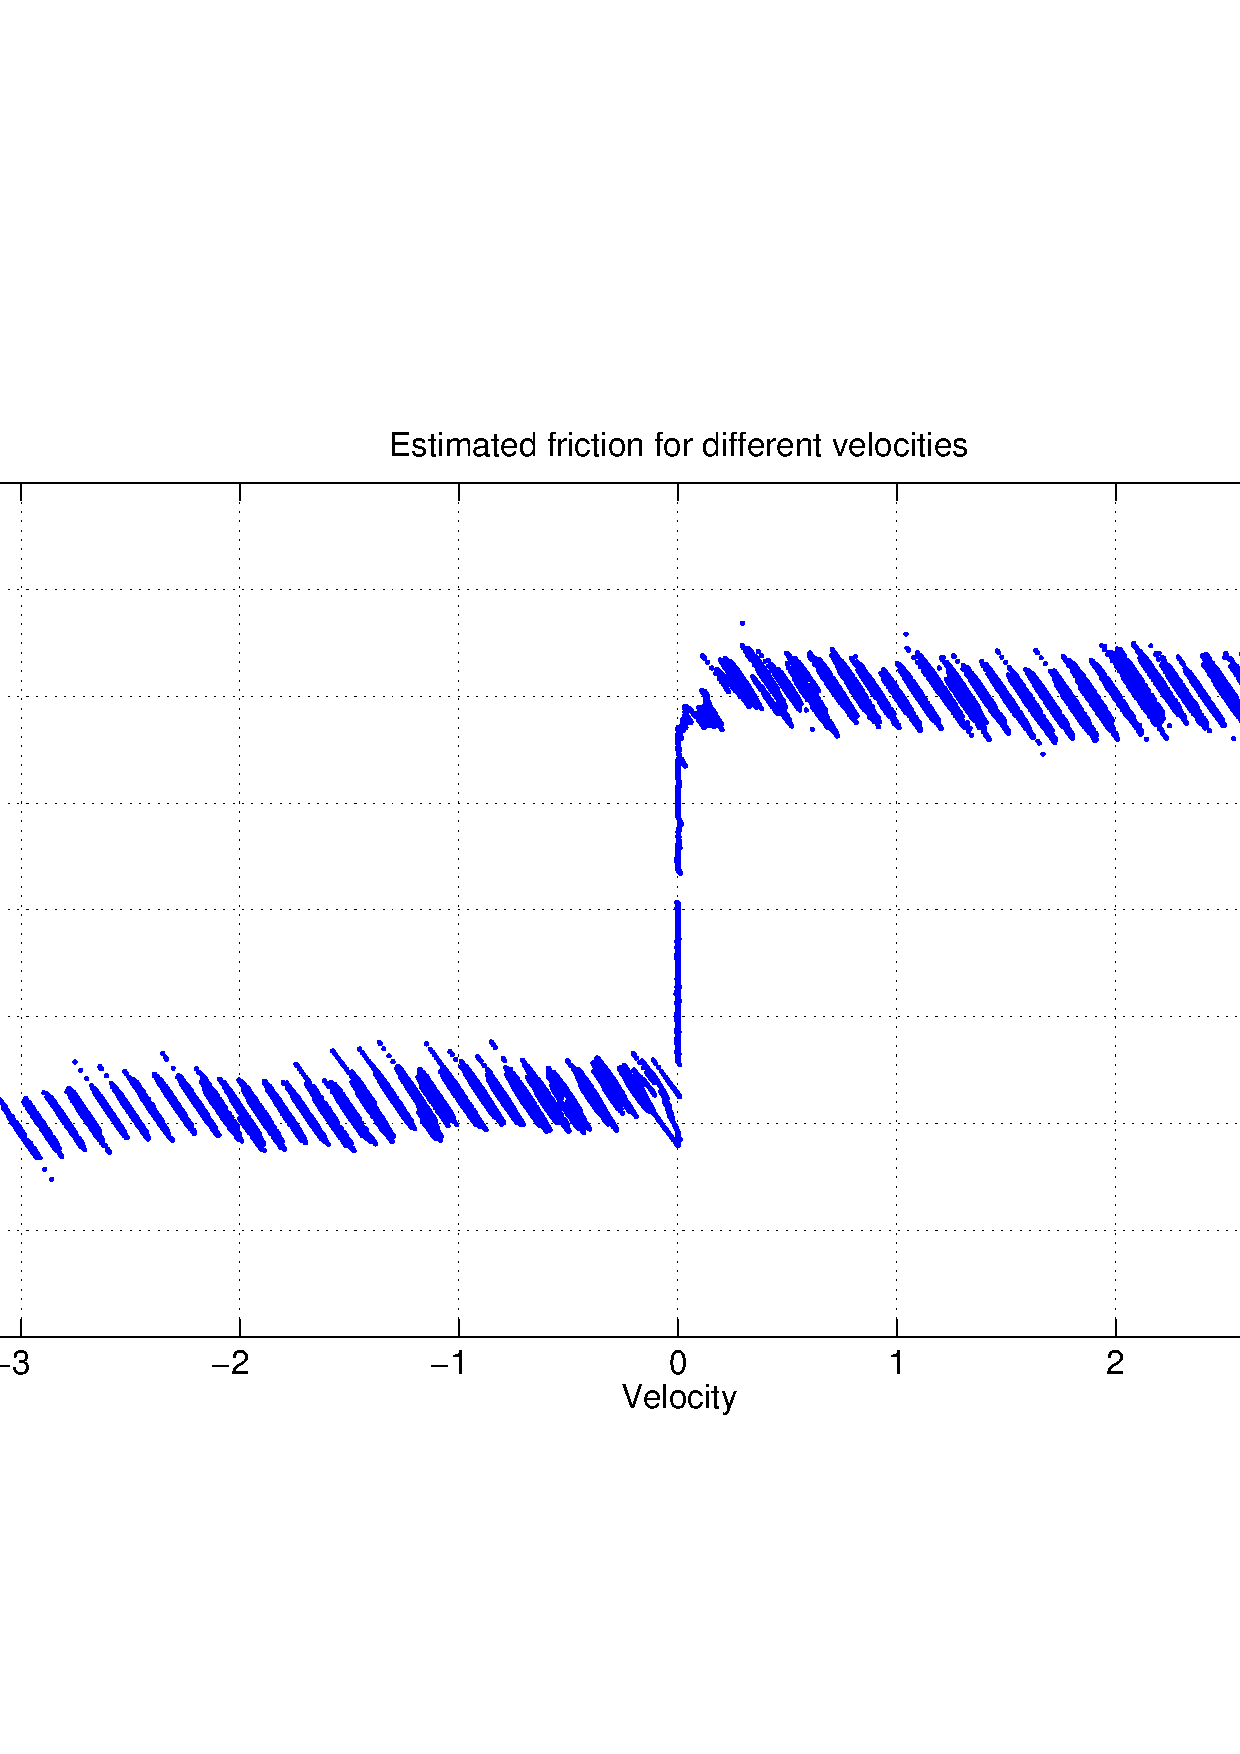
\includegraphics[width=1\textwidth]{fric.png}
\caption{Measured friction of the process for different velocities}
\label{fig:fric}
\end{center}
\end{figure}
\begin{figure}[!htb]
\begin{center}
\includegraphics[width=1\textwidth]{frictmodel.png}
\caption{a) Friction model with coulomb friction. b) Friction model with coulomb and viscous friction.}
\label{fig:frictmodel}
\end{center}
\end{figure}
\subsection{Friction estimation}
\label{sec:fricEst}
To manage the friction an estimate of a simple friction model is derived using RLS. The models in fig \ref{fig:frictmodel} will respectively give the following friction expressions 
\begin{equation}
 f=f_c\cdot sign(\dot{\varphi})
 \label{eq:f}
 \end{equation}
\begin{equation}
 f=f_c\cdot sign(\dot{\varphi})+f_v\cdot \dot{\varphi}
 \label{eq:fv}
 \end{equation}
where \ref{eq:f} is model a and only depends on the direction of the velocities and \ref{eq:fv} is the model in b where a viscous term that depends on the velocity is added.
 
The regression models for the two friction models will take the form of \ref{eq:regressor}.
\begin{equation}
\phi=sign(\dot{\varphi}), \beta = f_c
\label{eq:regressora}
\end{equation}
\begin{equation}
\phi=\begin{bmatrix}
sign(\dot{\varphi}) \\
\dot{\varphi}
\end{bmatrix}, \beta = \begin{bmatrix}
f_c\\
f_v
\end{bmatrix}
\label{eq:regressorb}
\end{equation}
Since the friction can be seen as a direct negative torque on the arm, it can be directly subtracted from the control signal which gives us the system in \ref{eq:discrete}
$$x_{k+1} = A_dx_k + B_d(u_k - f)$$
To get the RLS to work we take all measurements one step back in time and try to estimate the parameters from \ref{eq:regressor}. We also aim to use the measurement from the arm velocity where we get values from both the pendulum position and the arm velocity, see the state equation for $ \varphi $  in eq. \ref{eq:discrete}. After placing all known variables on the left hand side and we the following
\begin{equation}
\frac{\dot{\varphi}_k + 0.0059\theta_{k-1}-1.9125u_{k-1}-\dot{\varphi}_{k-1}}{-1.9125} = \begin{pmatrix}
f_c & f_v
\end{pmatrix}\begin{pmatrix}
\dot{\varphi}_{k-1}\\
sign(\dot{\varphi})
\end{pmatrix}
\label{eq:estim}
\end{equation}
Now we can apply the normal RLS algorithm with some forgetting factor $\lambda$.

As we see in equation \ref{eq:discrete} we probably can get different results in the friction estimation by choosing different equations in the same form as in equation \ref{eq:estim}. Initially we want to estimate the friction when the pendulum is hanging straight down and the arm is rotating at a constant speed. If there were no friction, no control signal would be necessary to keep the velocity of the arm constant, and therefore the control signal required corresponds to the signal necessary for compensating the coloumb friction.
We also want to to estimate the friction in the top position and then the equation corresponding to the state $ \dot{\varphi} $ in eq. \ref{eq:discrete} might not be the one which yields the best result. More research will be put into this at a later stage.

\subsection{RLS ALG}

\begin{equation}
\hat{\theta}_k = \hat{\theta}_{k-1}+P_k\phi_k\epsilon_k 
\end{equation}
\begin{equation}
\epsilon_k=y_k-\phi_k^{T}\hat{\theta}_{k-1} 
\end{equation}
\begin{equation}
P_k=\frac{1}{\lambda}(P_{k-1}-\frac{P_{k-1}\phi_k\phi_k^{T}P_{k-1}}{\lambda+\phi_k^{T}P_{k-1}\phi_k})
\end{equation}

\section{GUI}
The operator should be able to change controller parameters for both types of controller and for the friction estimator. For the top controller, the $Q$ and $R$ matrices. For the swing up controller, the switching area and its limit and the gain. Other general parameters for the controller such as sampling time $h$ (if possible), and $\omega _0$. And for the friction estimation the forgetting factor $\lambda$ and the initial values $P_0$ and $\omega _0$.

The GUI will plot the outputs from the Furuta pendulum, the friction estimation, control signal, both uncompensated as well as the compensated signal. We aim to have different regressor modes for the friction compensation and the operator can therefore change different parameters depending on the regressor chosen. 

\begin{figure}[!htb]
\begin{center}
\includegraphics[width=1\textwidth]{gui.png}
\caption{Overview of the program structure}
\label{fig:gui}
\end{center}
\end{figure}
\section{Results}

\section{Conclusion}


\end{document}

